\documentclass[10pt]{article}
\usepackage[margin=1in]{geometry}
\usepackage[T1]{fontenc}
\usepackage[utf8]{inputenc}
\usepackage{lmodern}
\usepackage{amsmath}
\usepackage{array}
\usepackage{booktabs}
\usepackage{caption}
\usepackage{enumitem}
\usepackage{graphicx}
\usepackage{hyperref}
\usepackage{xcolor}
\hypersetup{colorlinks=true,linkcolor=blue!50!black,citecolor=blue!50!black,urlcolor=blue!50!black}
\graphicspath{{figures/}}
\setlist{nosep,leftmargin=*}
\setlength{\parskip}{0.35em}
\setlength{\parindent}{0em}

\title{\textbf{Verification-Gated Model Cascading for Local Coding Inference}}
\author{Neeraj Pragnya Krishna Vasagiri\\Independent Researcher}
\date{29 August 2026\\\textit{Local preprint; not peer reviewed}}

\begin{document}
\maketitle

\begin{abstract}
Large language model routing is often evaluated as a cost-quality trade-off,
but model failures need not be nested: a smaller model can sometimes produce
a correct program when a larger model does not. This paper studies whether a
deterministic verifier can exploit that complementarity through a local
verification-gated cascade. We audit one completed experiment on 542 paired
EvalPlus tasks (164 HumanEval+ and 378 MBPP+) using same-family Qwen2.5-Coder
FAST, BALANCED, and BEST tiers. Adaptive produced 331 verified Plus successes
(61.07\%), compared with 297 (54.80\%) for Strong-only and 220 (40.59\%) for
Small-only. Its 34 additional successes over Strong-only came from FAST (22)
and BALANCED (12), with no additional BEST successes. The model-size-weighted
total-token cost proxy was 899,462.8 versus 893,000.0 (+0.72\%), while raw
total tokens (+121.04\%), CPU time (+14.11\%), and wall time (+65.40\%) were
higher. Successes per weighted total-token proxy were 10.65\% higher for
Adaptive, but successes per CPU second were slightly lower. These proxies are
not FLOPs, measured compute, energy, API usage, or dollar cost. The evidence
supports task-level complementarity and verification-gated escalation at this
operating point, not a universal efficiency advantage or a strong claim about
predictive initial routing.
\end{abstract}

\textbf{Keywords:} code generation, model cascading, LLM routing, verification,
EvalPlus, local inference, reproducibility

\section{Introduction}

Selecting one language model for every request is simple, but it can waste
capacity when tasks vary in difficulty. A smaller model may be adequate for
some tasks, while a larger model may be needed for others. More subtly, the
sets of tasks solved by two models need not be nested. A routing system can
benefit from this complementarity only if it has an authoritative way to decide
when an answer is acceptable.

This paper investigates a narrow, falsifiable question:
\begin{quote}
Can verification-gated model cascading exploit task-level complementarity among
differently sized language models to increase verified coding-task completion
efficiently relative to always using the strongest available model?
\end{quote}

The evaluated system is a local benchmark subsystem of Adaptive Workflow. It
starts with a local tier, generates one candidate, and runs deterministic
EvalPlus tests. A failed verification permits one escalation to the next tier.
The historical run did not transfer a failed program or verifier feedback into
the next prompt; later tiers received the original frozen task prompt. Thus,
the contribution studied here is a verification-gated model cascade, not
failure-feedback reasoning or collaborative error correction.

The primary historical result is task-weighted Plus correctness on the same
542 tasks: Adaptive passes 331 tasks (61.07\%), Strong-only passes 297
(54.80\%), and Small-only passes 220 (40.59\%). Adaptive has 34 successes not
present in Strong-only. Twenty-two of those final successes were produced by
FAST and twelve by BALANCED; BEST produced no additional Adaptive-only
successes. This is evidence that correctness sets are not nested by model
size, not evidence that a small model is stronger on average.

\subsection{Research questions}
\begin{description}
\item[RQ1.] Can a verification-gated multi-model cascade achieve more verified
coding-task successes than always using the strongest available model?
\item[RQ2.] To what extent are improvements explained by task-level
complementarity among differently sized models?
\item[RQ3.] What additional expenditure does the cascade incur under raw
tokens, model-size-weighted token proxies, CPU, memory, and wall time?
\item[RQ4.] How much evidence does the completed experiment provide for
adaptive initial routing beyond a simpler verification-gated cascade?
\end{description}

\section{Related Work}
\subsection{Model routing and cascades}
FrugalGPT describes prompt adaptation, model approximation, and LLM cascades,
including settings with improved accuracy at the same reported API cost
\cite{chen2024frugalgpt}. RouteLLM learns a preference-data router to select
between stronger and weaker models \cite{ong2025routellm}. Early-abstention
cascades use correlated errors to avoid some expensive calls
\cite{zellinger2025abstention}. These studies motivate query-dependent model
choice, but differ from this work's local same-family models and deterministic
code verifier.

Faster Cascades via Speculative Decoding interleaves models through speculative
execution \cite{narasimhan2025cascades}; speculative decoding uses a small
model to propose tokens and a larger model to verify them
\cite{leviathan2023speculative}. Adaptive Workflow is sequential: each program
is accepted or rejected by tests, and no speculative token verification occurs.

\subsection{Adaptive inference and test-time computation}
Confident Adaptive Language Modeling allocates computation within a model using
confidence-calibrated early exits \cite{schuster2022calm}. Snell et al. show
that prompt difficulty can make adaptive test-time allocation more effective
than uniform scaling \cite{snell2024testtime}. We follow their methodological
lesson of separating measured hardware quantities from approximate accounting:
parameter-weighted token values are proxies, while CPU, RAM, and time are
physical observations.

\subsection{Verification for code generation}
HumanEval introduced function-level code synthesis tasks scored by executing
generated Python \cite{chen2021humaneval}. MBPP provides short programming
problems for entry-level synthesis \cite{austin2021mbpp}. EvalPlus augments
original tests to expose test insufficiency \cite{liu2023evalplus}. We use
HumanEval+ and MBPP+ as deterministic verification views. Self-Debugging uses
execution feedback to revise programs \cite{chen2023selfdebug}; our historical
cascade deliberately did not pass failure context to later tiers. Self-
consistency samples multiple paths \cite{wang2023selfconsistency}; our one
deterministic completion per tier does not estimate pass@k.

\section{Adaptive Workflow}
\subsection{System overview}
For a task $x$, the system selects an initial tier, obtains a completion $y$,
and invokes a deterministic verifier $V(x,y)$. If $V$ passes, $y$ is retained.
If it fails, the fixed historical policy permits one attempt at the next tier:
FAST $\rightarrow$ BALANCED $\rightarrow$ BEST. Infrastructure failures are
recorded and are not retried into a pass.

\begin{figure}[t]
\centering
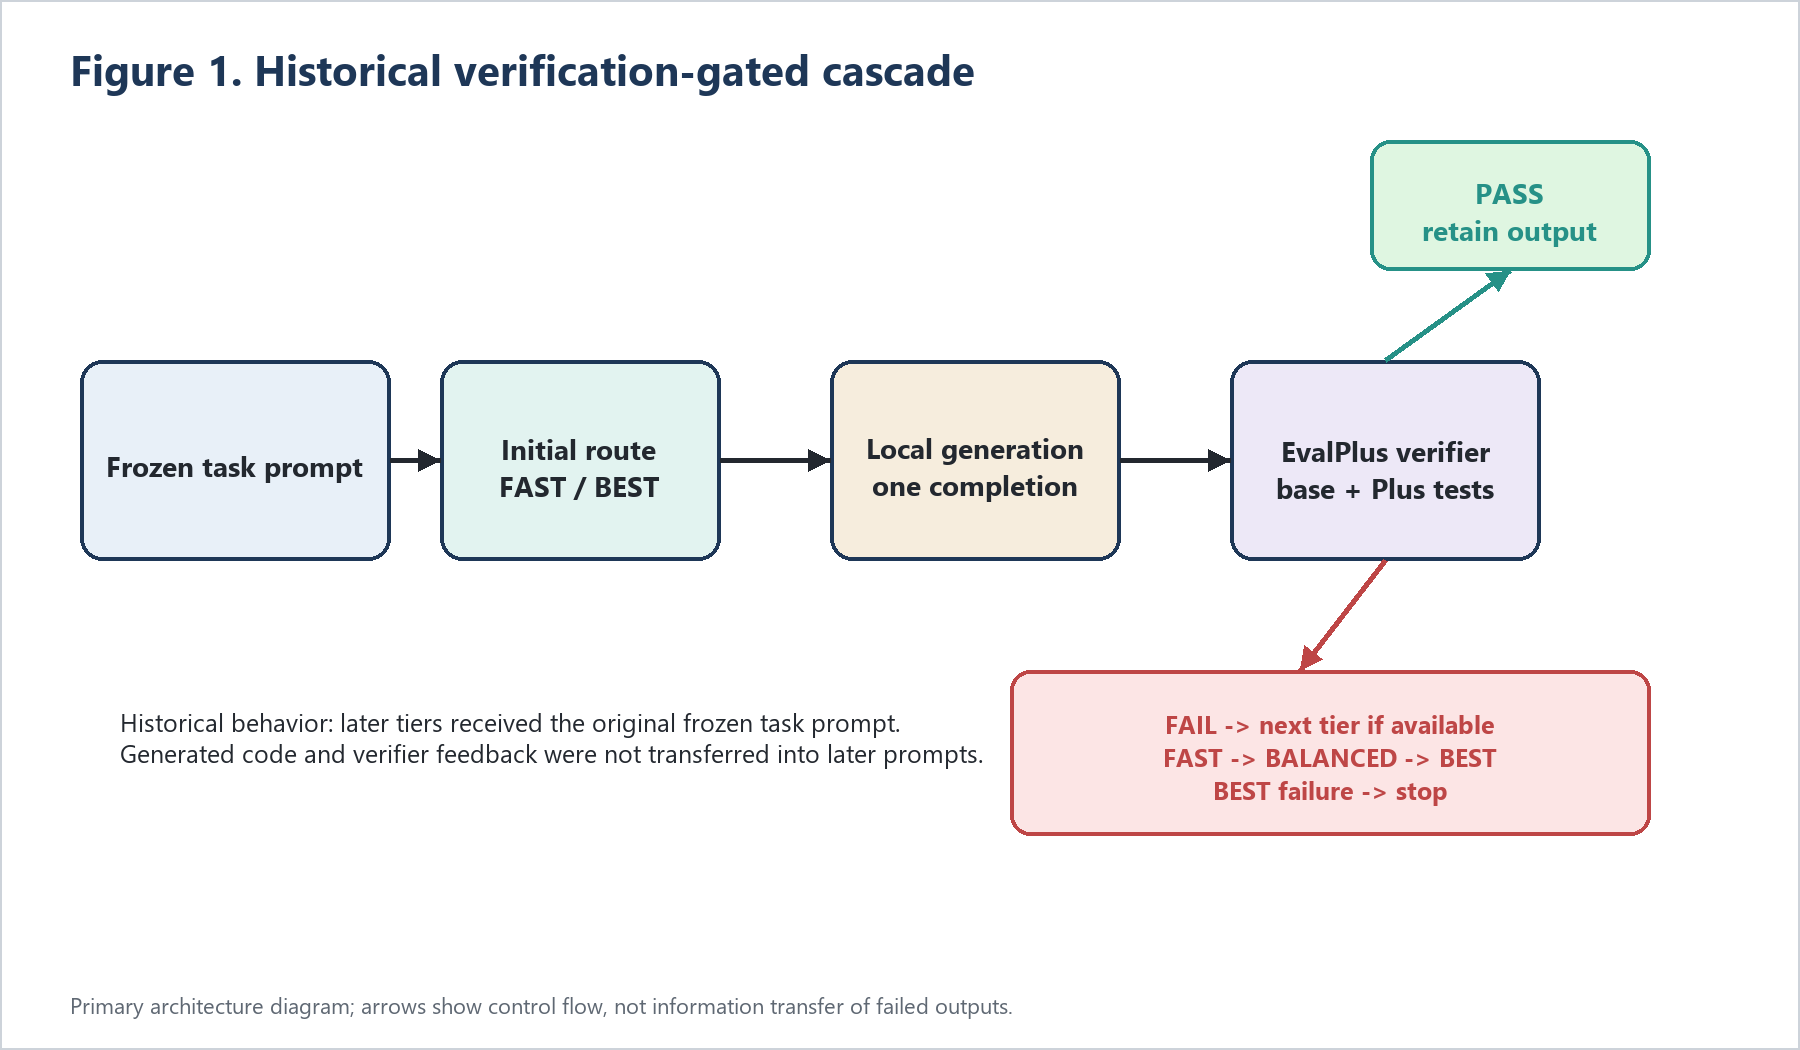
\includegraphics[width=\linewidth]{figure1_architecture.png}
\caption{Historical verification-gated cascade. A pass terminates the cascade;
a failure permits escalation. Later tiers received the original frozen task
prompt, not the failed program or verifier feedback.}
\label{fig:architecture}
\end{figure}

\subsection{Tiers, routing, and verification}
The manifest maps FAST, BALANCED, and BEST to qwen2.5-coder:1.5b,
qwen2.5-coder:3b, and qwen2.5-coder:7b. Frozen parameter values are 1.5,
3.1, and 7.6 billion, all Q4\_K\_M. The manifest records model sizes and
SHA-256 digests. Initial Adaptive routing selected FAST for 531 of 542 tasks,
BEST for 11, and BALANCED for zero. The audit's chronological online replay
has no mismatches; an empty-state replay differs on eight history-dependent
HumanEval decisions.

EvalPlus ran in the pinned image
\texttt{ganler/evalplus:v0.3.1@sha256:26b118098bef281fe8dfe999bf05f1d5b45374b4e6c00161ec0f30592aef4740}
with network disabled, a read-only root, dropped capabilities, an
unprivileged user, task-scoped temporary storage, a PID cap, a 120-second
timeout, and one verifier worker.

\section{Experimental Method}
\subsection{Tasks and conditions}
The primary set contains 164 HumanEval+ and 378 MBPP+ tasks. HumanEval was
pinned to commit
\texttt{6d43fb980f9fee3c892a914eda09951f772ad10d}; MBPP to
\texttt{f46ca8374b4cddef97ca4208ad986049d74d296a}; EvalPlus to v0.3.1;
HumanEval+ to v0.1.10; and MBPP+ to v0.2.0. The same 542 task IDs and order
were used for Small-only, Strong-only, and Adaptive. Base and Plus are two
scores of each completion, not 1,084 independent observations.

\begin{table}[t]
\centering
\scriptsize
\caption{Frozen benchmark configuration. Full model and artifact metadata are
in the repository manifest.}
\label{tab:configuration}
\begin{tabular}{llll}
\toprule
Item & Frozen value & Size/count & Notes \\
\midrule
HumanEval+ & v0.1.10 & 164 & EvalPlus augmented tests \\
MBPP+ & v0.2.0 & 378 & EvalPlus augmented tests \\
Total & same paired task set & 542 & one completion scored on base and Plus \\
FAST & qwen2.5-coder:1.5b & 1.5B & Q4\_K\_M \\
BALANCED & qwen2.5-coder:3b & 3.1B & Q4\_K\_M \\
BEST & qwen2.5-coder:7b & 7.6B & Q4\_K\_M \\
Sampling & temperature 0; top\_p 1 & seed 20260824 & one thread; 1024 output cap \\
Verifier & EvalPlus & v0.3.1 & Docker network none; 120 s timeout \\
Resource ceiling & CPU 45\% soft / 50\% hard & RAM 45\% soft / 50\% hard & process-tree controls \\
\bottomrule
\end{tabular}

\end{table}

\subsection{Generation and resource protocol}
Temperature was 0, top-$p$ was 1, the seed was 20260824, the context window
was 8,192, the output cap was 1,024, and one model thread was used. The
machine reported 25,652,355,072 bytes of physical RAM. Resource controls
targeted 45\% and hard-limited 50\% of total CPU capacity and physical RAM.
The CPU equivalent in the manifest is only a readability aid, not a fractional
CPU assignment. RAM soft and hard limits were 11,543,559,782 and
12,826,177,536 bytes. No cap violation was recorded.

\subsection{Metrics and fixed budget}
For a tier with frozen parameter value $P$ in billions, we define
$C_{\mathrm{generation}}=P\times\mathrm{output\_tokens}$ and
$C_{\mathrm{total}}=P\times(\mathrm{input\_tokens}+\mathrm{output\_tokens})$.
These are model-size-weighted token cost proxies, not measured FLOPs,
hardware compute, energy, API usage, credits, or dollar cost. Physical
evidence is measured CPU time/utilization, wall time, RAM, peak RAM,
model-load time, inference time, and verification time.

Before the run, the frozen total-token baseline was $B_0=4,818,407.6$ with
cutoffs 1,204,601.9, 2,409,203.8, 3,613,805.7, and 4,818,407.6. Every
condition exhausted its task list before the first cutoff. We preserve this
predeclared definition and label its resulting curves nondiscriminating;
condition-relative curves are post-hoc diagnostics.

\subsection{Statistical analysis and reproducibility}
Paired task-level outcomes are retained. The exact two-sided McNemar test was
computed after the run and is labeled post-hoc. The frozen source hash is
\texttt{0d24437e9297466c3f28a7af677a76d7e54c10dc6358edb7b724d586040e7859}.
The private raw JSONL and SQLite hashes are recorded in the audit. The
historical run retained exact prompts privately, verifier output, and model
metadata, but not exact generated programs or generated-program hashes.
This paper is calculation-reproducible, not exact-output-reproducible for the
old run.
The McNemar calculation treats the 542 fixed benchmark task pairs as the
observational units; no population sampling frame or out-of-benchmark
generalization is claimed.

\section{Results}
\subsection{Overall correctness}
\begin{table}[t]
\centering
\scriptsize
\caption{Primary task-weighted and equal-benchmark-macro Plus pass rates.}
\label{tab:correctness}
\begin{tabular}{lrrrr}
\toprule
Condition & HumanEval+ & MBPP+ & Overall & Macro average \\
\midrule
Small-only & 26/164 (15.85\%) & 194/378 (51.32\%) & 220/542 (40.59\%) & 33.59\% \\
Strong-only & 34/164 (20.73\%) & 263/378 (69.58\%) & 297/542 (54.80\%) & 45.15\% \\
Adaptive & 43/164 (26.22\%) & 288/378 (76.19\%) & 331/542 (61.07\%) & 51.20\% \\
\bottomrule
\end{tabular}

\end{table}

Adaptive passes 331 of 542 tasks (61.07\%), compared with 297 (54.80\%) for
Strong-only and 220 (40.59\%) for Small-only. Equal-benchmark macro averages
are 51.20\%, 45.15\%, and 33.59\%, respectively.

\begin{figure}[t]
\centering
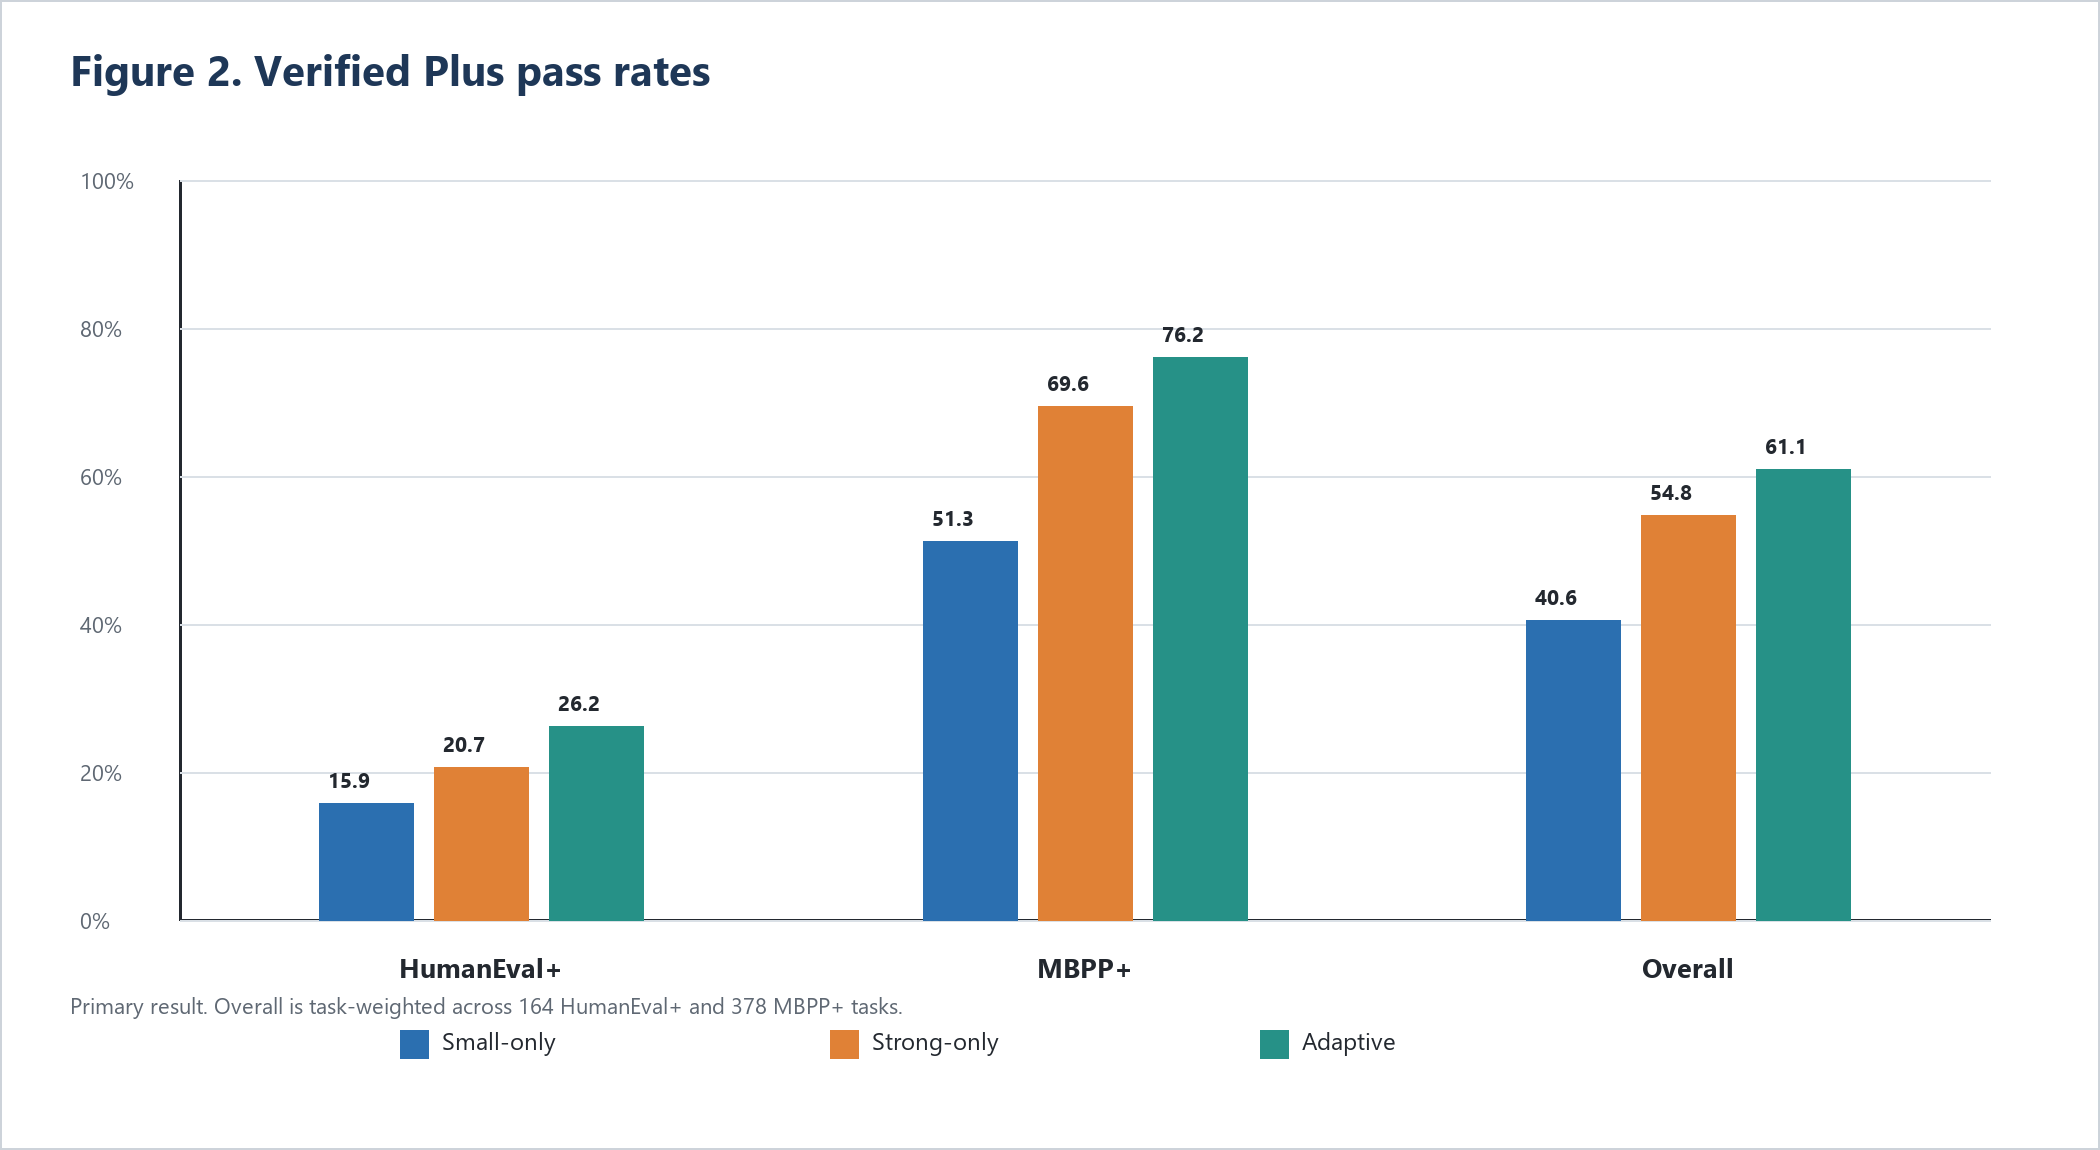
\includegraphics[width=\linewidth]{figure2_plus_pass_rates.png}
\caption{Primary verified Plus pass rates. Overall is task-weighted across
HumanEval+ and MBPP+; Base and Plus are not independent samples.}
\label{fig:passrates}
\end{figure}

\subsection{Adaptive versus Strong-only}
Adaptive has 34 additional verified Plus successes, a paired risk difference
of 6.27 percentage points and a relative increase of 11.45\% in successful
tasks. There are 297 tasks passing in both conditions, 34 passing only under
Adaptive, none passing only under Strong-only, and 211 failing in both. The
exact two-sided McNemar p-value is
$1.1641532182693481\times10^{-10}$; this post-hoc statistic does not establish
generalization beyond this task set.

\begin{table}[t]
\centering
\scriptsize
\caption{Adaptive versus Strong-only expenditure and physical measurements.
Relative differences use Strong-only as denominator.}
\label{tab:resources}
\begin{tabular}{lrrr}
\toprule
Metric & Adaptive & Strong-only & Relative difference \\
\midrule
Plus successes & 331 & 297 & +11.45\% \\
Raw input tokens & 166,716 & 78,993 & +111.05\% \\
Raw output tokens & 93,006 & 38,507 & +141.53\% \\
Raw total tokens & 259,722 & 117,500 & +121.04\% \\
Weighted input proxy & 579,460.70 & 600,346.80 & -3.48\% \\
Weighted output proxy & 320,002.10 & 292,653.20 & +9.35\% \\
Weighted total proxy & 899,462.80 & 893,000 & +0.72\% \\
CPU seconds & 38,137.61 & 33,421.46 & +14.11\% \\
Wall seconds & 78,701.93 & 47,582.32 & +65.40\% \\
Peak CPU & 47.12 & 46.89 & +0.235 pp \\
Peak RAM bytes & 6,897,147,346 & 6,999,388,192 & -1.46\% \\
Model calls & 1,092 & 542 & +101.48\% \\
Verifier calls & 1,091 & 542 & +101.29\% \\
\bottomrule
\end{tabular}

\end{table}

\begin{table}[t]
\centering
\scriptsize
\caption{Paired Adaptive versus Strong-only outcomes. The test is post-hoc.}
\label{tab:paired}
\begin{tabular}{lr}
\toprule
Paired outcome & Count \\
\midrule
Both pass & 297 \\
Adaptive only & 34 \\
Strong-only only & 0 \\
Both fail & 211 \\
\midrule
Paired risk difference & 6.27\% \\
Exact McNemar p-value (post-hoc) & 1.164e-10 \\
\bottomrule
\end{tabular}

\end{table}

\subsection{Complementary successes and escalation}
The 34 Adaptive-only successes comprise 22 FAST outputs and 12 BALANCED
outputs; BEST contributes zero additional successes. Among all 331 Adaptive
successes, 216 (65.26\%) ended at FAST, 69 (20.85\%) at BALANCED, and 46
(13.90\%) at BEST. Thus 285 of 331 successes (86.10\%) avoided BEST. This
does not mean FAST or BALANCED is stronger overall: the static FAST-versus-
BEST comparison has 22 FAST-only passes, 99 BEST-only passes, 198 in both,
and 223 failures in both.

\begin{figure}[t]
\centering
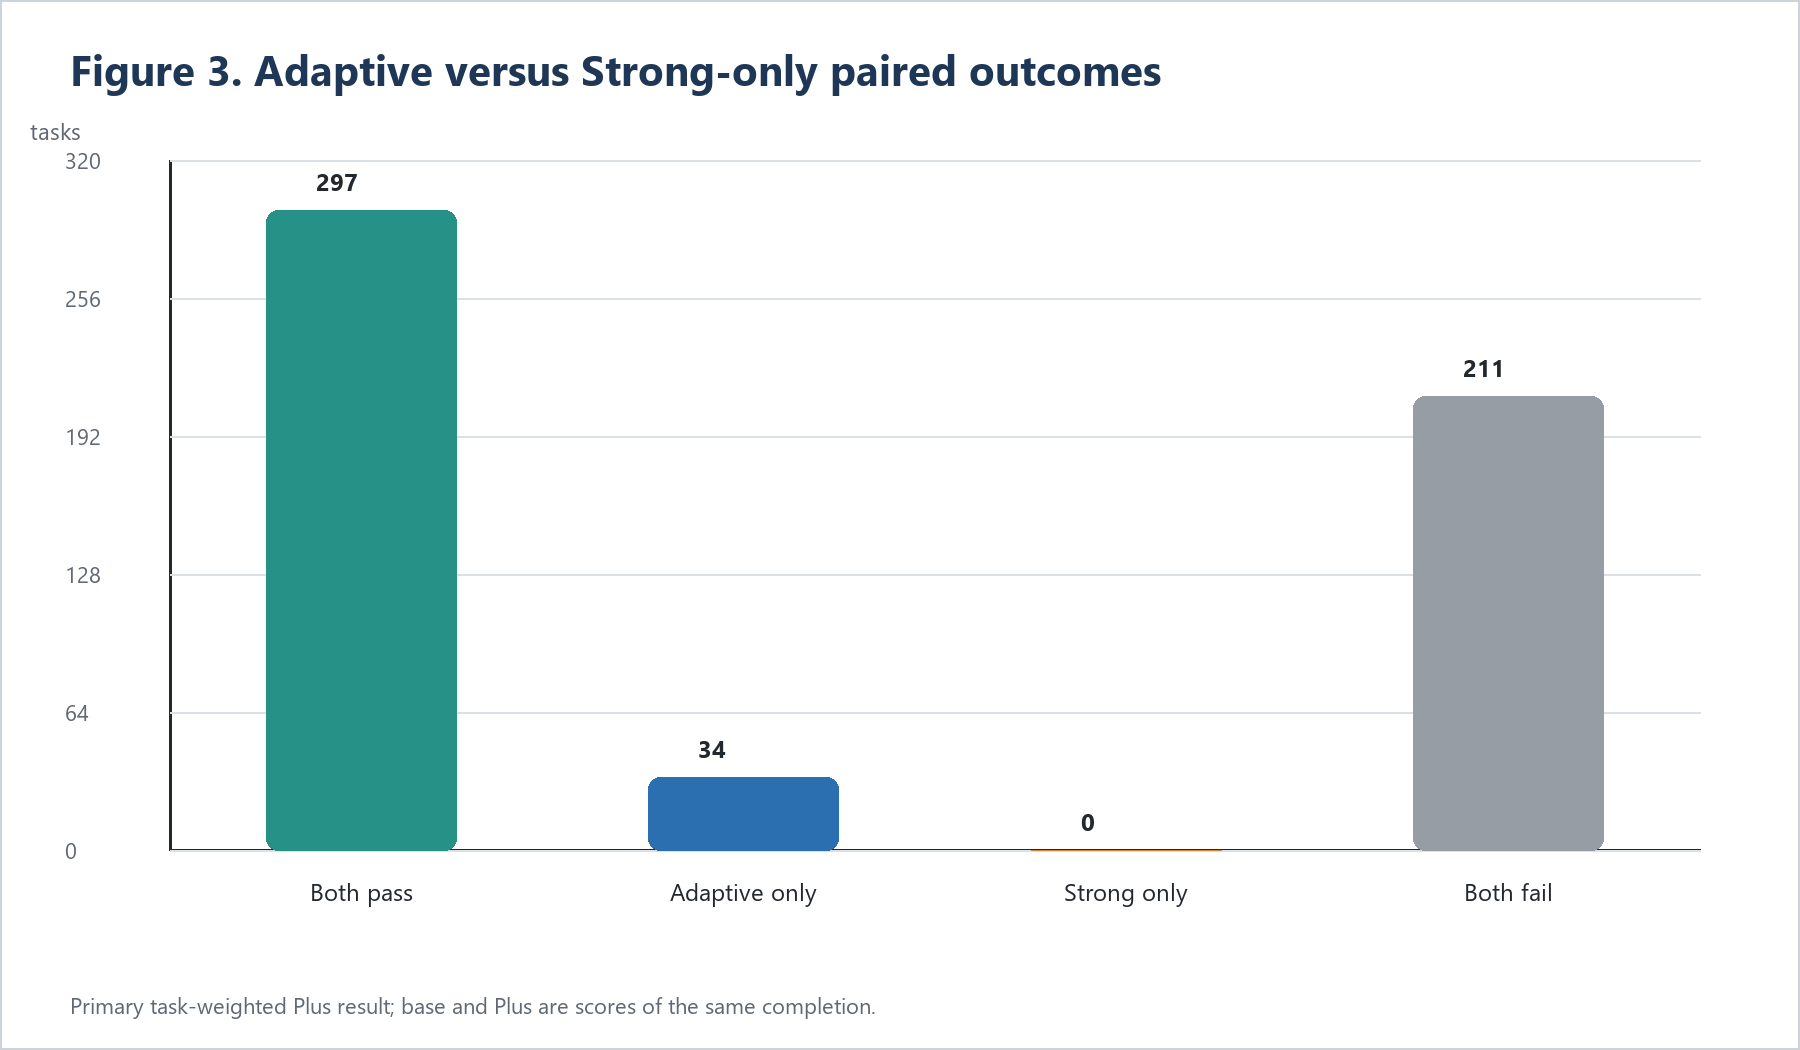
\includegraphics[width=\linewidth]{figure3_paired_outcomes.png}
\caption{Primary paired outcomes for Adaptive and Strong-only.}
\label{fig:paired}
\end{figure}

\begin{figure}[t]
\centering
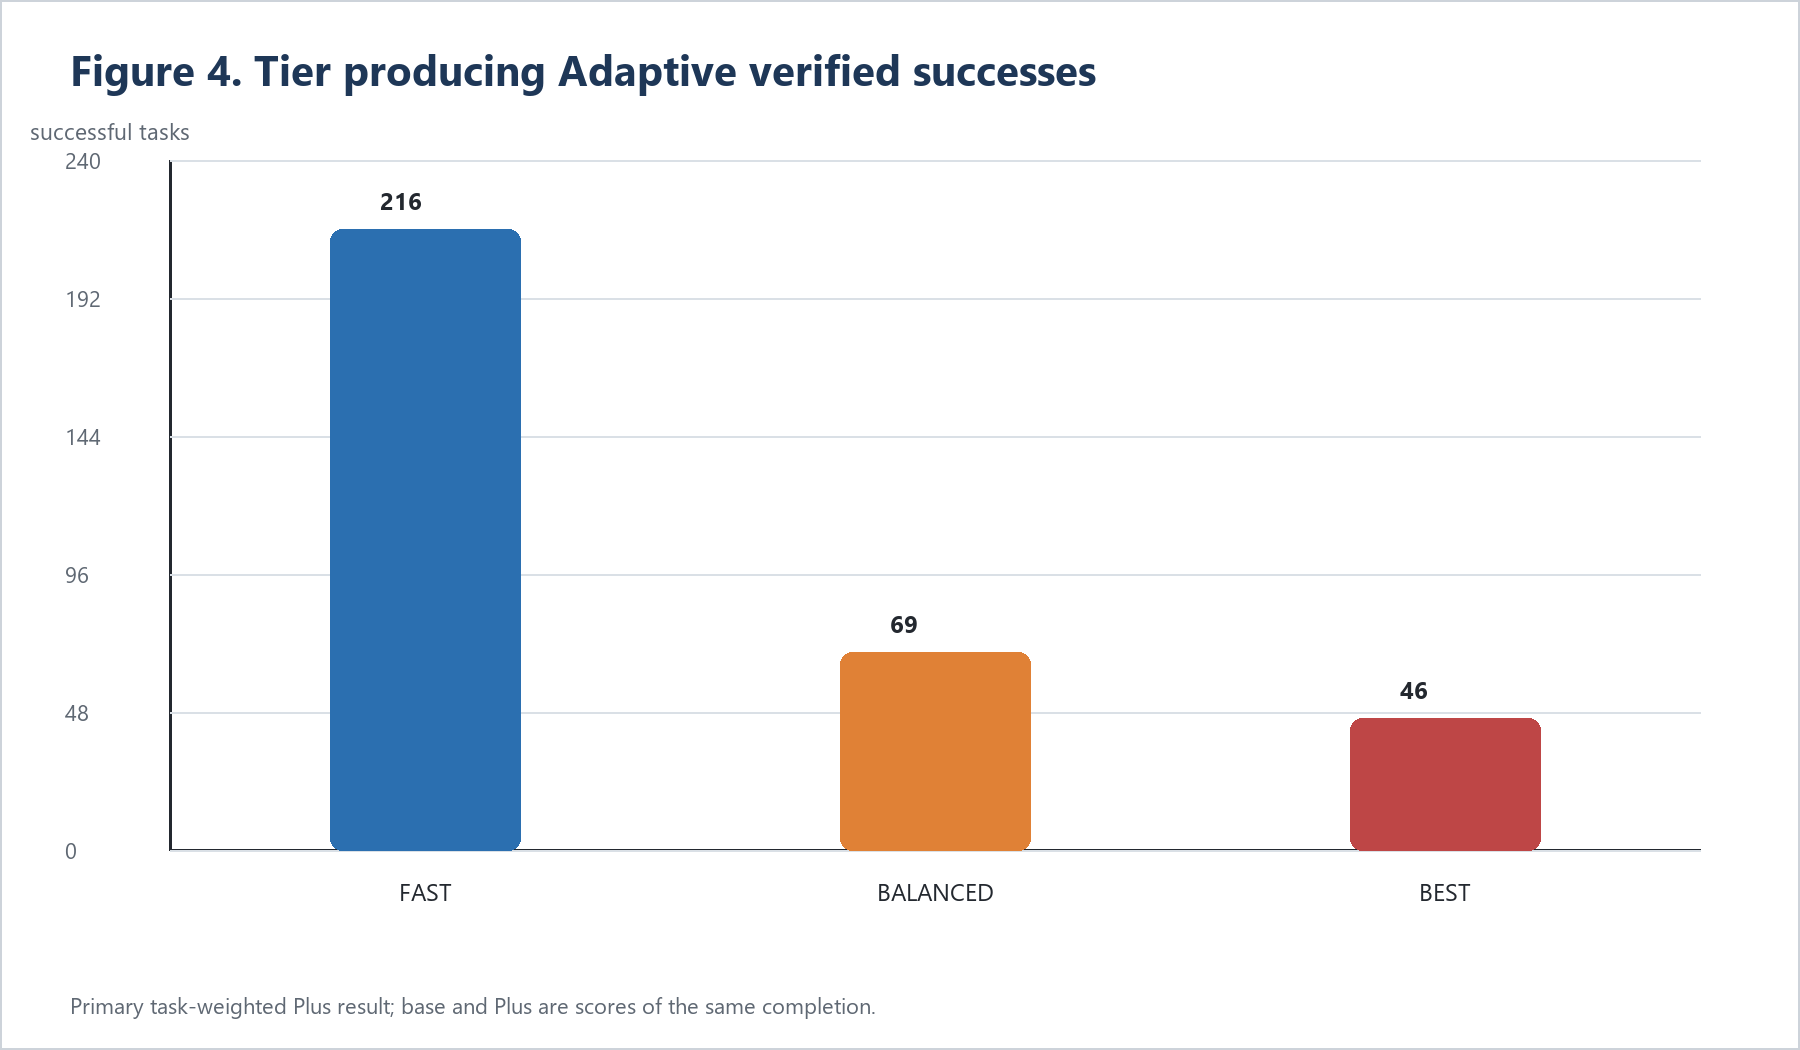
\includegraphics[width=\linewidth]{figure4_success_tiers.png}
\caption{Primary source tier for final verified Adaptive successes.}
\label{fig:tiers}
\end{figure}

\begin{table}[t]
\centering
\scriptsize
\caption{Observed conditional tier overlaps. These rows are not standalone
542-task Balanced or BEST baselines.}
\label{tab:complementarity}
\begin{tabular}{lrrrrr}
\toprule
Observed comparison & n & Both pass & A only & B only & Both fail \\
\midrule
FAST vs BALANCED (conditional) & 310 & 0 & 0 & 69 & 241 \\
BALANCED vs BEST (conditional) & 240 & 0 & 0 & 41 & 199 \\
FAST vs BEST static & 542 & 198 & 22 & 99 & 223 \\
Adaptive vs Strong-only & 542 & 297 & 34 & 0 & 211 \\
\bottomrule
\end{tabular}

\end{table}

Observed escalation paths were FAST only for 221 tasks, FAST to BALANCED for
70, FAST to BALANCED to BEST for 240, and BEST only for 11. There were 550
escalations. The initial distribution (FAST 531, BALANCED 0, BEST 11) means
the experiment strongly tests verification-gated escalation and
complementarity, but provides weaker evidence for sophisticated initial
predictive routing.

\begin{figure}[t]
\centering
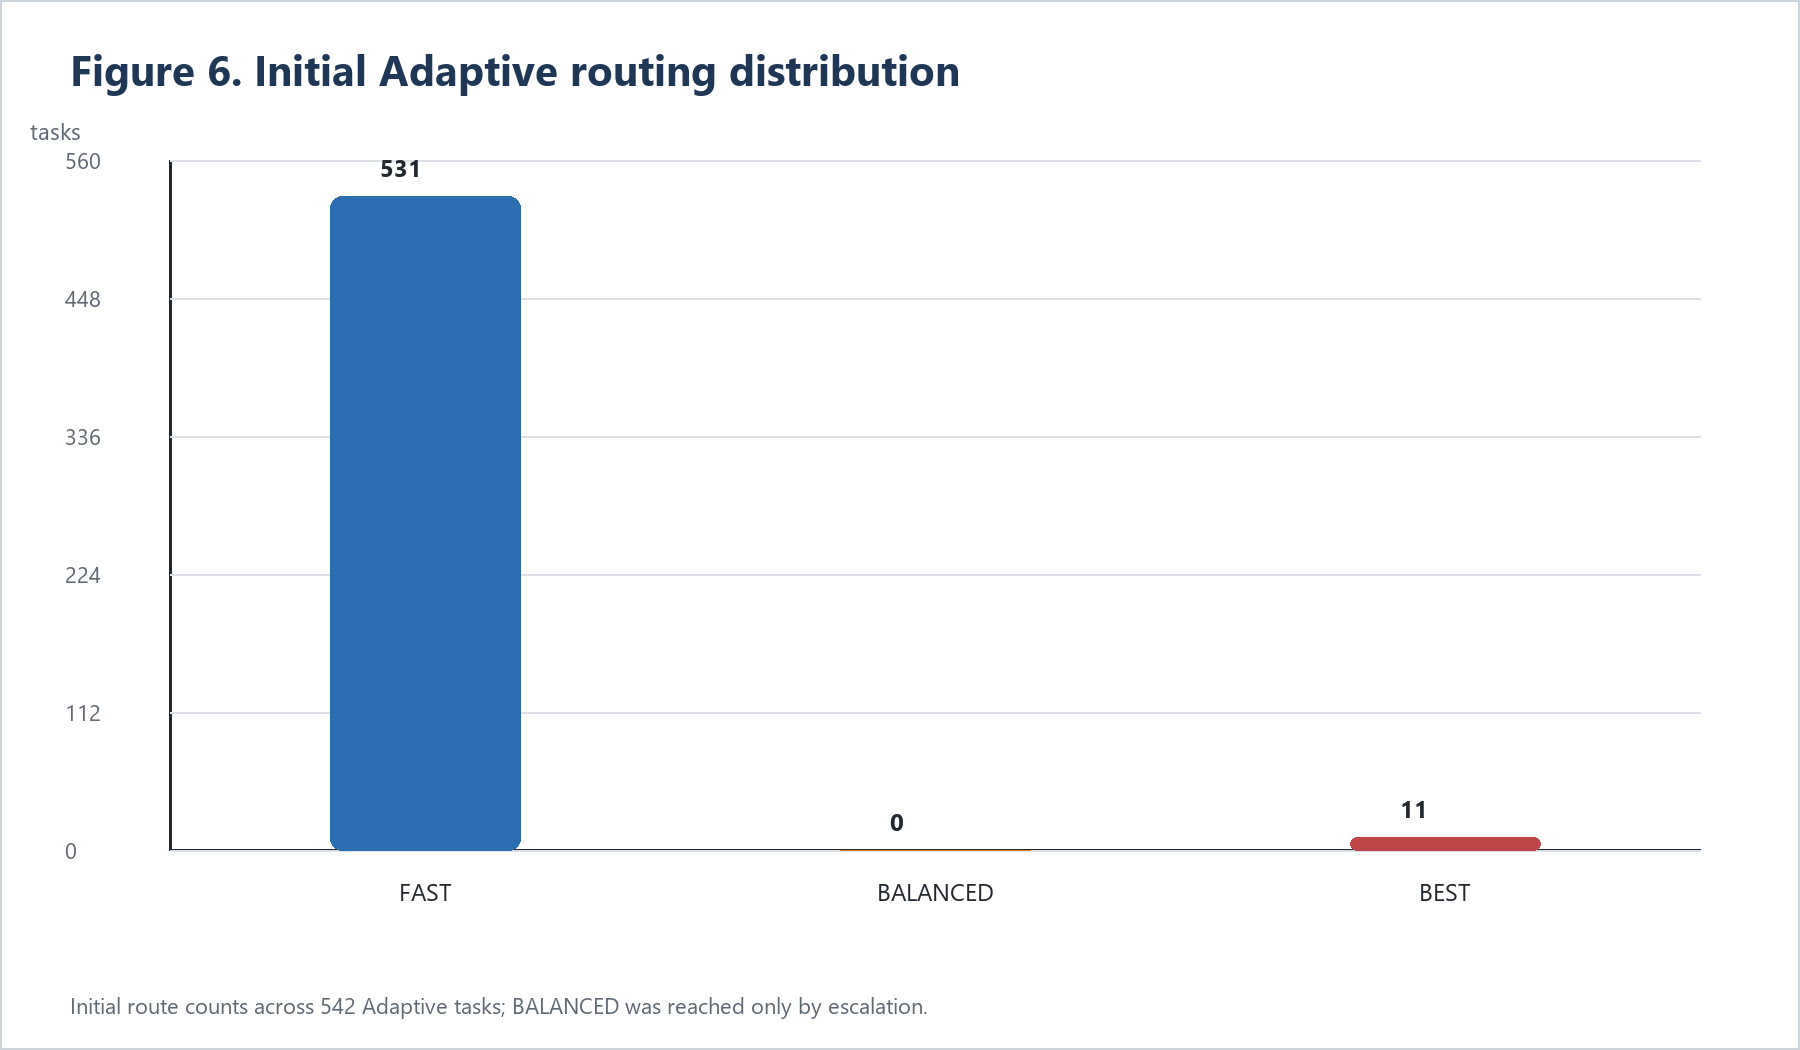
\includegraphics[width=\linewidth]{figure6_initial_routing.png}
\caption{Primary initial Adaptive routing distribution. BALANCED was reached
mainly through escalation.}
\label{fig:routing}
\end{figure}

\subsection{Resource and usage trade-offs}
Adaptive used 1,092 model calls and 1,091 verifier calls versus 542 and 542
for Strong-only. Raw input tokens were 166,716 versus 78,993 (+111.05\%);
raw output tokens were 93,006 versus 38,507 (+141.53\%); and raw total tokens
were 259,722 versus 117,500 (+121.04\%). Weighted input-token proxy was lower
for Adaptive (579,460.7 versus 600,346.8, -3.48\%), weighted output was higher
(320,002.1 versus 292,653.2, +9.35\%), and weighted total-token proxy was
899,462.8 versus 893,000.0 (+0.72\%).

Successes per weighted total-token proxy were 0.0003679974 for Adaptive and
0.0003325868 for Strong-only, a 10.65\% relative improvement in this one
proxy-normalized measure. CPU time was 38,137.61 versus 33,421.46 seconds
(+14.11\%); wall time was 78,701.93 versus 47,582.32 seconds (+65.40\%).
Peak CPU was 47.1225\% versus 46.8875\%; peak RAM was 6,897,147,346 versus
6,999,388,192 bytes. The mixed metrics rule out a universal efficiency score.

\begin{figure}[t]
\centering
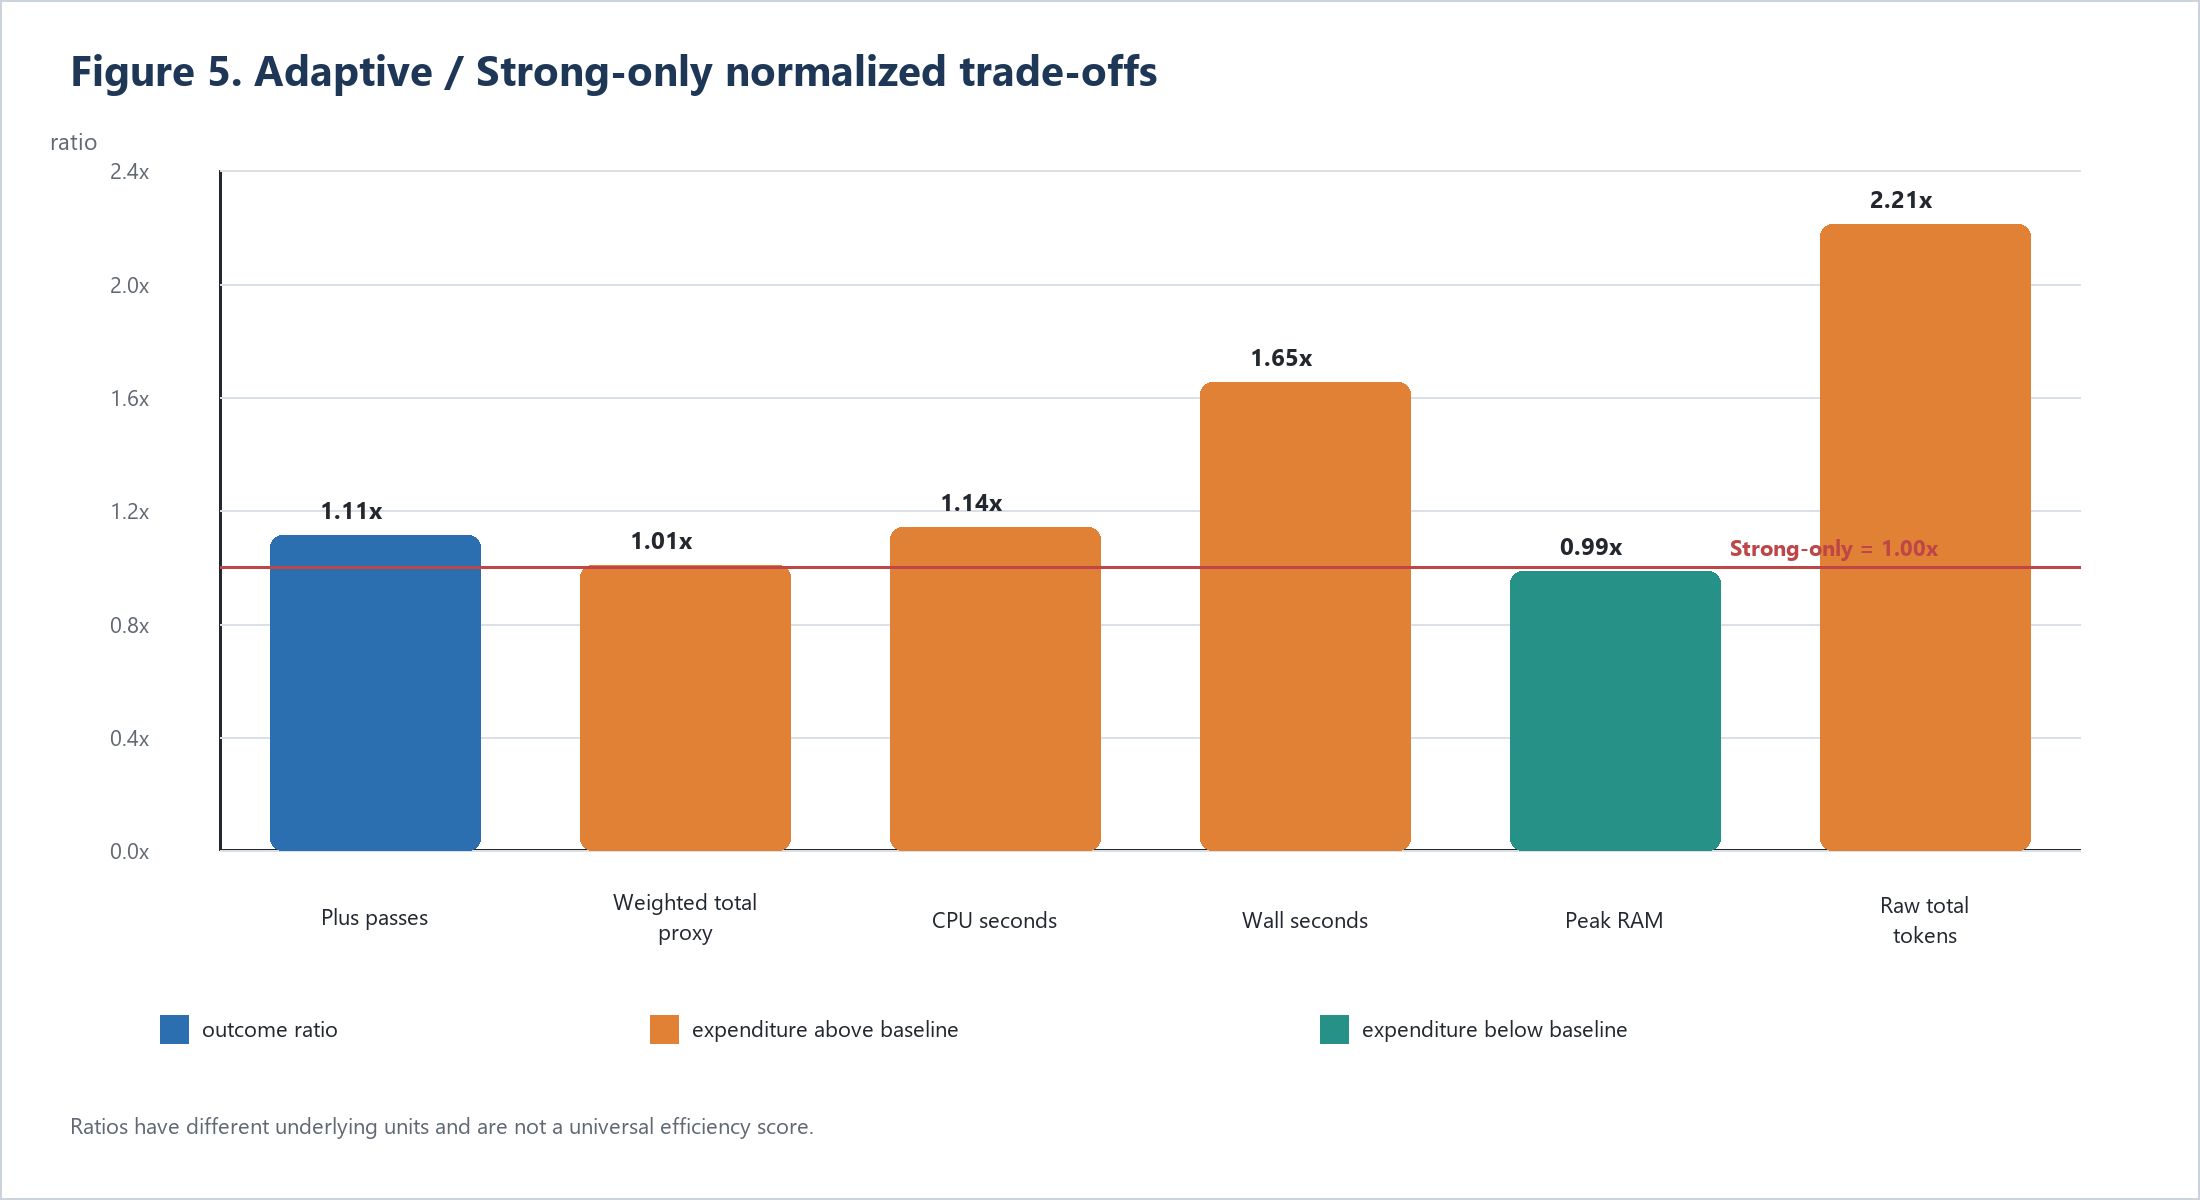
\includegraphics[width=\linewidth]{figure5_tradeoffs.png}
\caption{Primary normalized trade-offs. Each bar is a separate ratio to
Strong-only; unlike units are not combined into one score.}
\label{fig:tradeoffs}
\end{figure}

\subsection{Post-hoc diagnostics}
Six MBPP tasks generated shared verifier/infrastructure failures in all three
conditions: Mbpp/106, Mbpp/124, Mbpp/252, Mbpp/255, Mbpp/580, and Mbpp/720.
The primary result retains them in the denominator. Excluding them
post-hoc gives Adaptive 331/536 (61.75\%), Strong-only 297/536 (55.41\%),
and Small-only 220/536 (41.04\%). These do not replace the primary values.
The predeclared frozen budget curve is nondiscriminating because the first
cutoff is at or above every condition's actual expenditure; condition-relative
curves remain post-hoc diagnostics.

\section{Analysis}
\subsection{Why the cascade gains successes}
The paired outcomes show that Adaptive retains 297 tasks also solved by
Strong-only and adds 34 tasks that Strong-only misses. Deterministic
verification accepts a passing FAST or BALANCED completion immediately, so a
correct smaller-model output is not discarded merely because a larger model
could be invoked. The result is consistent with a union of non-nested
correctness sets, not with making BEST more capable.

\subsection{Verification, conditional tiers, and routing}
The static FAST-versus-BEST comparison measures both endpoints for all 542
tasks, while BALANCED and later BEST outcomes are conditional on earlier
failures. The conditional rows are descriptive, not standalone tier accuracy
estimates. Verification is an execution gate, not a learned judge. Because no
failure message entered a later prompt, this is not failure-feedback repair.
The heavily FAST initial route and eight empty-state replay differences show
online adaptation but limited evidence for predictive initial routing.

\subsection{Efficiency interpretation}
Adaptive's 0.72\% increase in weighted total-token proxy accompanies a 10.65\%
increase in successes per proxy unit. Raw tokens, model calls, CPU time, and
wall time favor Strong-only more clearly. The weighted input proxy is slightly
lower for Adaptive, but output and tier weights make the total proxy slightly
higher. These are different quantities; physical measurements remain the
primary evidence for hardware efficiency.

\section{Limitations}
\begin{table}[t]
\centering
\scriptsize
\caption{Threats to validity and treatment.}
\label{tab:threats}
\begin{tabular}{p{0.32\linewidth}p{0.58\linewidth}}
\toprule
Threat & Treatment in this study \\
\midrule
Oracle gate & The same finite EvalPlus Plus result controlled escalation and the endpoint; no independent verifier is evaluated. \\
Attempt asymmetry & Adaptive could retain earlier-tier passes and fall back to BEST; repeated-model and fixed-cascade baselines are absent. \\
Conditional tiers & Label tier overlaps as observed conditional outcomes; no standalone Balanced baseline is claimed. \\
Online selection & Routing statistics updated during evaluation; task order and earlier test labels could affect later routes. \\
Verifier failures & Keep six shared MBPP infrastructure failures in the primary denominator; exclusion is post-hoc. \\
Budget curve & Preserve frozen B0 and disclose that every condition exhausted before the first cutoff. \\
Output retention & State that exact historical generated programs were not persisted. \\
Public benchmark age & Treat contamination as plausible and avoid general-intelligence claims. \\
Proxy interpretation & Call weighted token values proxies, never FLOPs or generic compute. \\
\bottomrule
\end{tabular}

\end{table}
\begin{enumerate}
\item One deterministic run on one Windows machine; physical measurements are
not portable cost guarantees.
\item HumanEval and MBPP are old public benchmarks; contamination is plausible.
\item One same-family model set was tested; family, quantization, runtime, and
hardware effects may change complementarity.
\item There was no historical Balanced-only condition or fixed-cascade ablation.
\item The router updated statistics online and was not tested frozen on a
held-out set.
\item Exact historical generated programs and hashes were not retained.
\item Six shared verifier failures remain in the primary denominator.
\item Frozen $B_0$ cutoffs exceed actual expenditure and do not discriminate.
\item Token proxies are not FLOPs, energy, API price, or generic resource use.
\item One deterministic completion per task does not estimate pass@k or variance.
\item Function-level Python tasks do not measure repository-scale engineering
or general intelligence.
\end{enumerate}

\section{Future Work}
Future work should add a complete Balanced-only baseline, a fixed cascade
ablation, a frozen-router held-out evaluation, multiple seeds, multiple model
families, newer or private coding tasks, and exact private output hashes.
Further studies could test deterministic failure-context extraction, compressed
failure memory, context-aware escalation, and provider-specific real-cost
measurements. Any feedback-driven repair mechanism should be a new condition.

\section{Conclusion}
In this completed local experiment, verification-gated cascading produced 331
verified Plus successes versus 297 for Strong-only and 220 for Small-only on
the same 542 tasks. The 34 Adaptive-only successes came from FAST and
BALANCED outputs, not from making BEST more capable. The result is consistent
with non-nested task-level correctness and with verification retaining correct
smaller-model outputs before escalation.

The expenditure picture is mixed: weighted total-token proxy +0.72\% and
success-per-proxy +10.65\%, but raw tokens, model calls, CPU time, and wall
time increase. The defensible conclusion is bounded: this operating point
shows a verification-gated local cascade exploiting model complementarity,
not universal superiority, a FLOPs saving, or improved model intelligence.

\section*{AI assistance disclosure}
AI systems, including ChatGPT and Codex, assisted with transforming the
author's ideas and recorded results into academic prose, organization,
editing, formatting, and code/audit assistance. They did not originate the
architecture, research direction, benchmark result, or scientific
conclusions. The author reviewed the manuscript and retains responsibility for
the research and final version.

\bibliographystyle{plain}
\bibliography{references}

\appendix
\section{Audit details}
The audit reports 2,176 attempt records from 1,626 completed condition-task
cells and zero duplicate attempt keys. It records raw hashes, source hashes,
model digests, sampling settings, verification configuration, resource
extrema, and one token-telemetry reconciliation. Private prompts, generated
programs, raw logs, databases, and model files are absent from the public
bundle.

\section{Failure taxonomy}
Adaptive attempts include 331 verified passes, 351 model-incorrect, 98
test-failure, 305 timeout, 6 verifier-infrastructure, and 1 resource-blocked
records. Strong-only includes 297 passes, 105 model-incorrect, 39 test-failure,
95 timeout, and 6 verifier-infrastructure records. Small-only includes 220
passes, 184 model-incorrect, 31 test-failure, 101 timeout, and 6
verifier-infrastructure records. These categories are descriptive.

\end{document}
